% Source printed pp. 466-475 / PDF pp. 474-483.
\section{半稳定约化, 模空间与分层}\label{src:9.3}
\begin{epigraph}
代数是魔鬼向数学家提出的交易. 魔鬼说: ``我给你这台强大的机器; 它会回答你想问的任何问题. 你只需把灵魂交给我: 放弃几何, 你就能拥有这台奇妙的机器.''
\epigraphauthor{Michael Atiyah \cite[第 7 页]{Ati02}}
\end{epigraph}
我们证明曲线上向量丛模叠的进一步性质: 半稳定轨迹 $\cBun_{r,d}^{\mathrm{ss}}$ 普遍闭 (定理~\bookref{9.3.1}), 并有固有模空间 (定理~\bookref{9.3.11}); 不稳定轨迹 $\cBun_{r,d}\setminus\cBun_{r,d}^{\mathrm{ss}}$ 则有以 Harder--Narasimhan 多边形为指标的分层 (定理~\bookref{9.3.15}).
\subsection{半稳定约化: Langton 定理}\label{src:9.3.1-subsection}
\begin{theorem}[Langton 定理]\label{src:9.3.1}
设 $C$ 是代数闭域 $\Bbbk$ 上亏格 $g\geq2$ 的光滑连通射影曲线. 设 $R$ 是 $\Bbbk$ 上的 DVR, 分式域为 $K$. 若 $E^*$ 是 $C_K$ 上半稳定向量丛, 则存在 $C_R$ 上的半稳定向量丛族 $E$, 使得 $E_K\cong E^*$.
\end{theorem}
\begin{remark}\label{src:9.3.2}
一般代数叠的赋值判据的存在性部分需要对 $R$ 作基变换 (见例~\bookref{4.8.17}--\bookref{4.8.19} 和 \bookref{6.5.11}), 此处则不需要基变换.
\end{remark}
\begin{proof}
可假设 $R/\pi\cong\Bbbk$,\footnote{事实上, 当 $\Bbbk$ 为任意域时, 此定理也成立, 证明相同.} 其中 $\pi$ 为一致化元. 令 $r=\operatorname{rk}(E^*)$, $d=\deg(E^*)$. 由 $\cBun_{r,d}$ 的赋值判据 (习题~\bookref{4.8.14}), 存在 $C_R$ 上向量丛 $E$, 满足 $E_K\cong E^*$. 策略是通过``初等修改''修改 $E$, 使 $E_{\Bbbk}$ 半稳定. 具体地, 若 $E_{\Bbbk}$ 不半稳定, 则可选取短正合列
\begin{equation*}\tag{$\star$}\label{src:9.3-langton-star}
0\to D\to E_{\Bbbk}\to F\to0,
\end{equation*}
使得 $F$ 在 $F$ 的最小斜率的半稳定商中最大, 即 $D$ 是 $E_{\Bbbk}$ 的 Harder--Narasimhan 滤过的最后一项; 见图~\bookref{9.3.3}.\footnote{如 Langton 的证明, 可以修改论证, 改取 $D\subseteq E_{\Bbbk}$ 为最大不稳定化子层, 即 $E_{\Bbbk}$ 的 Harder--Narasimhan 滤过的第一项.} 定义\newterm{初等修改}{elementary modification}
\[
E':=\ker(E\twoheadrightarrow E_{\Bbbk}\twoheadrightarrow F)\subseteq E.
\]
由构造, $E_K'\cong E_K\cong E^*$ 且 $E/E'\cong F$. 包含关系 $\pi E\subseteq E'\subseteq E$ 蕴含 $E'/\pi E\cong D$, 这是利用短正合列 \eqref{src:9.3-langton-star} 中的等同得到的:
\[
0\to\underbrace{E'/\pi E}_D\to\underbrace{E/\pi E}_{E_{\Bbbk}}\to\underbrace{E/E'}_F\to0.
\]
有短正合列
\begin{equation*}\tag{$\star\star$}\label{src:9.3-langton-double-star}
0\to F\to E_{\Bbbk}'\to D\to0,
\end{equation*}
其中 $D,F$ 的角色与 \eqref{src:9.3-langton-star} 相反. 这是由满射 $E_{\Bbbk}'\cong E'/\pi E'\twoheadrightarrow E'/\pi E\cong D$ 及其核 $F\cong\pi E/\pi E'$ 得到的.\footnote{还可从另一角度理解此设置. 回顾 \S\bookref{7.9.2-subsection}, $\Phi_R:=[\Spec(R[s,t]/(st-\pi))/\mathbb G_m]$, 且 $\Phi_R\setminus0\cong\Spec R\bigcup_{\Spec K}\Spec R$ 是不分离 DVR. 因为 $E\bigcup_{E^*}E'$ 定义 $C\times(\Phi_R\setminus0)$ 上的族, 且 $\Coh(C)$ S-完备 (命题~\bookref{7.9.30}), 此族延拓为 $\Phi_R$ 上的族 $\mathcal F$. 此时可利用习题~\bookref{7.9.16} 的描述, 将它显式写为 $C_R$ 上的 $\mathbb Z$-分次层 $\mathcal F=\bigoplus_{n\in\mathbb Z}\mathcal F_n$, 带有如下图中的映射 $s,t$:
\[
\begin{tikzcd}[ampersand replacement=\&,column sep=small]
\cdots\arrow[r,bend left=20,"s"]\&\mathcal F_{-2}\arrow[l,bend left=20,"t"]\arrow[r,bend left=20,"{s=\pi}"]\arrow[d,equal]\&\mathcal F_{-1}\arrow[l,bend left=20,"{t=1}"]\arrow[r,bend left=20,"{s=1}"]\arrow[d,equal]\&\mathcal F_0\arrow[l,bend left=20,"{t=\pi}"]\arrow[r,bend left=20,"{s=1}"]\arrow[d,equal]\&\mathcal F_1\arrow[l,bend left=20,"{t=\pi}"]\arrow[r,bend left=20,"s"]\arrow[d,equal]\&\cdots\arrow[l,bend left=20,"t"]\\
\&E'\&E'\&E\&E\&{}
\end{tikzcd}
\]
正合列 \eqref{src:9.3-langton-star} 和 \eqref{src:9.3-langton-double-star} 分别对应沿 $t=0$ 和 $s=0$ 限制到 $\Theta_{\Bbbk}$ 所得的滤过.}

设 $\operatorname{HNP}(E_{\Bbbk})\subseteq\mathbb C$ 为 $E_{\Bbbk}$ 的 Harder--Narasimhan 多边形, 即当 $E'\subseteq E_{\Bbbk}$ 遍历满足 $\mu(E')>d/r$ 的所有子层时, 点 $Z(E')=-\deg(E')+\operatorname{rk}(E')i\in\mathbb C$ 的凸包.
\bookfiguretarget{9.3.3}
\begin{figure}[H]
\centering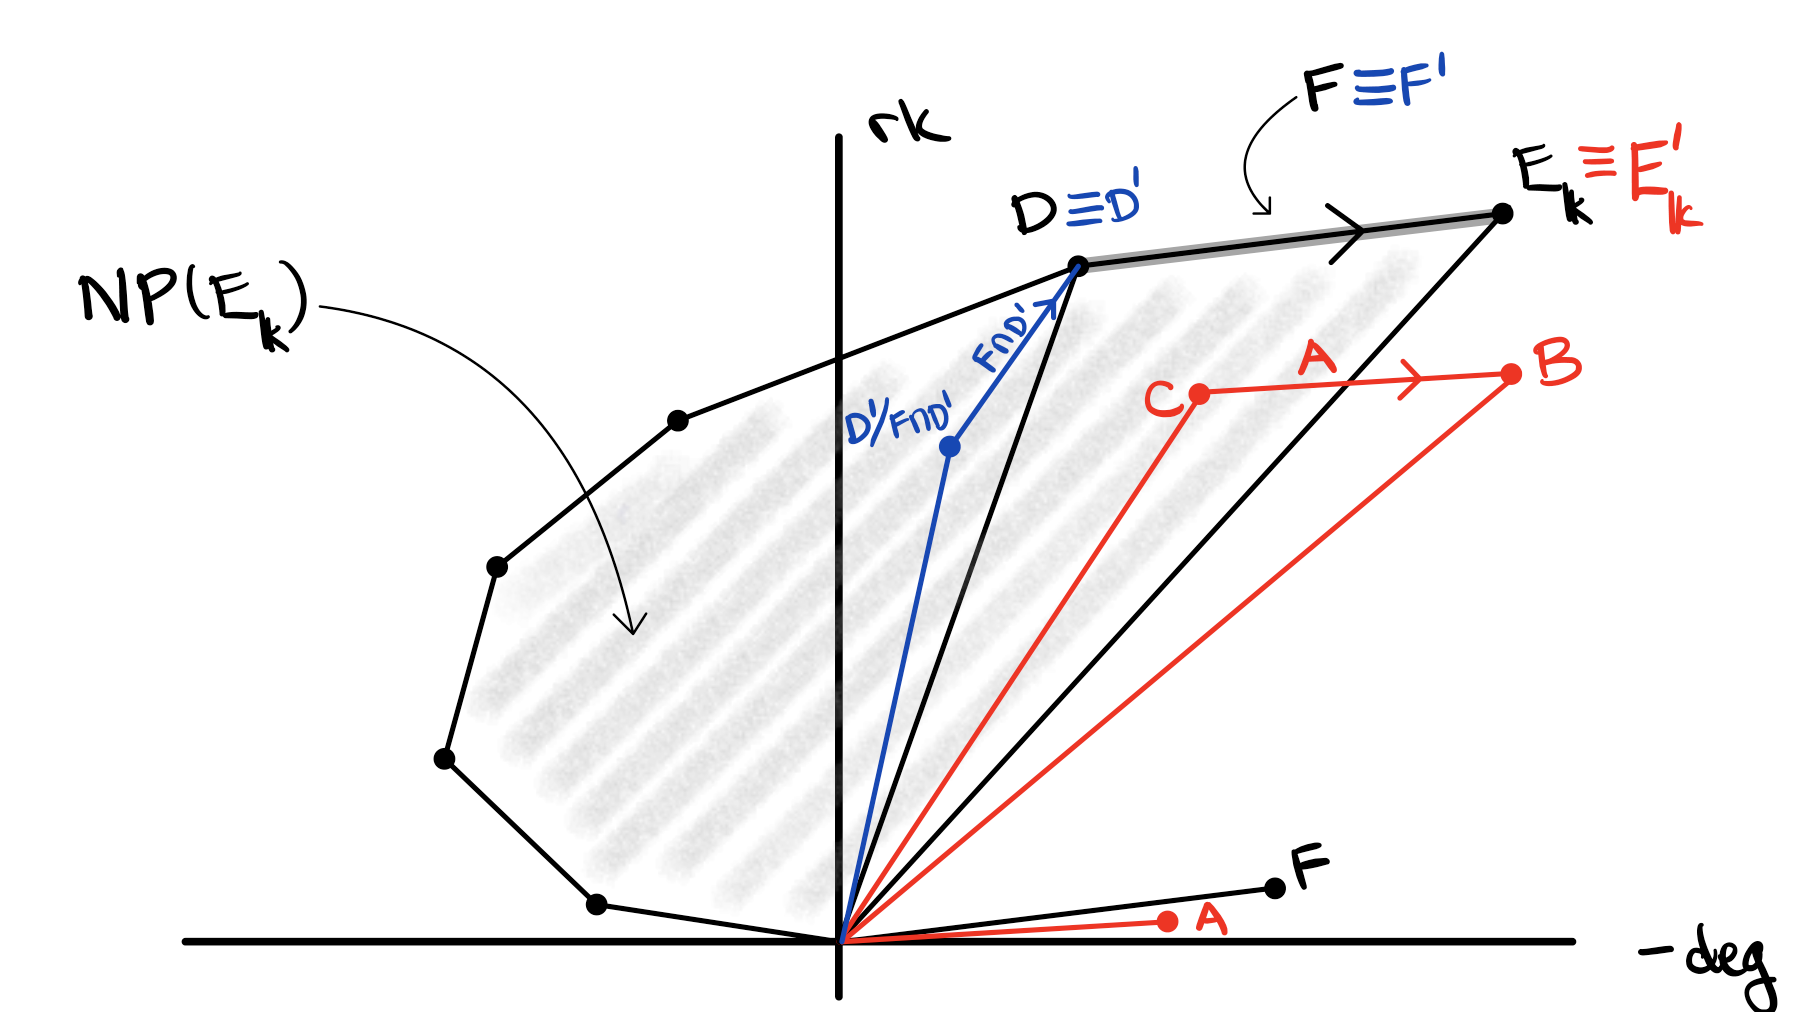
\includegraphics[width=0.76\textwidth]{figures/ch09-langton-polygon.png}
\bookfigurehref{9.3.3}
\caption{$E_{\Bbbk}$ 的 Harder--Narasimhan 多边形 $\operatorname{HNP}(E_{\Bbbk})$ 以灰色表示. 红色 (分别地, 蓝色) 向量用于说明包含关系 $\operatorname{HNP}(E_{\Bbbk}')\subseteq\operatorname{HNP}(E_{\Bbbk})$ 的证明 (分别地, 等号成立时 \eqref{src:9.3-langton-double-star} 的分裂).}\label{src:9.3.3}
\end{figure}
仿照对 $E_{\Bbbk}$ 构造 \eqref{src:9.3-langton-star} 的过程, 令 $0\to D'\to E_{\Bbbk}'\to F'\to0$ 为取 $D'$ 为 $E_{\Bbbk}'$ 的 Harder--Narasimhan 滤过的最后一项所得的短正合列. 我们断言:
\begin{enumerate}[(i)]
\item $\operatorname{HNP}(E_{\Bbbk}')\subseteq\operatorname{HNP}(E_{\Bbbk})$;
\item 若 $\operatorname{HNP}(E_{\Bbbk}')=\operatorname{HNP}(E_{\Bbbk})$, 则复合 $F\to E_{\Bbbk}'\to F'$ 和 $D'\to E_{\Bbbk}'\to D$ 为同构. 特别地, \eqref{src:9.3-langton-double-star} 分裂.
\end{enumerate}
对 (i), 子层 $B\subseteq E_{\Bbbk}'$ 诱导短正合列的交换图
\[
\begin{tikzcd}[ampersand replacement=\&,column sep=small]
0\arrow[r]\&A\arrow[r]\arrow[d]\&B\arrow[r]\arrow[d]\&C\arrow[r]\arrow[d]\&0\\
0\arrow[r]\&F\arrow[r]\&E_{\Bbbk}'\arrow[r]\&D\arrow[r]\&0.
\end{tikzcd}
\]
因为 $C\subseteq D\subseteq E_{\Bbbk}$, 有 $\mu(C)\leq d/r$ 或 $Z(C)\in\operatorname{HNP}(E_{\Bbbk})$. 因为 $F$ 半稳定, 若 $A\ne0$, 则 $\mu(A)\leq\mu(F)$. 利用 $Z(B)=Z(A)+Z(C)$, 这两个事实蕴含 $\mu(B)\leq d/r$ 或 $Z(B)\in\operatorname{HNP}(E_{\Bbbk})$.

对 (ii), 有短正合列 $0\to D'\to E_{\Bbbk}'\to F'\to0$, 满足 $Z(F')=Z(F)$. 复合 $F\to E_{\Bbbk}'\to F'$ 的核为 $D'\cap F$, 它处于短正合列
\[
0\to F\cap D'\to D'\to D'/F\cap D'\to0
\]
中. 假设 $F\cap D'\ne0$, 则 $F$ 的半稳定性以及 $F=E_{\Bbbk}/D$ 和 $D'\subseteq E_{\Bbbk}'$ 的构造给出不等式
\[
\mu(F\cap D')\leq\mu(F)<\mu(E_{\Bbbk})=\mu(E_{\Bbbk}')<\mu(D'),
\]
从而蕴含 $\mu(D'/F\cap D')>\mu(D')$. 因为 $D'/F\cap D'\subseteq D\subseteq E_{\Bbbk}$, $Z(D'/F\cap D')\in\operatorname{HNP}(E_{\Bbbk})$ 位于 $Z(D')$ 的左侧. 但这蕴含 $\mu(F\cap D')>\mu(F)$, 与 $F$ 的半稳定性矛盾. 所以 $F\cap D'=0$, $F\to E_{\Bbbk}'\to F'$ 单射. 因为 $F,F'$ 的次数与秩相同, $F\to F'$ 是同构, 使 \eqref{src:9.3-langton-double-star} 分裂.

由于包含于 $\operatorname{HNP}(E_{\Bbbk})$ 的 Harder--Narasimhan 多边形只有有限个, 归纳地用 $E'$ 替换 $E$ 并应用断言 (i), 要么得到延伸 $E^*$ 的半稳定向量丛族, 要么得到无限族 $\cdots\subseteq E^{(2)}\subseteq E^{(1)}\subseteq E^{(0)}$, 其中每个 $E^{(n)}$ 都有相同的 Harder--Narasimhan 多边形. 我们将说明后一情形导致矛盾. 由断言 (ii), 每个 $E_{\Bbbk}^{(n)}\cong D\oplus F$ 分裂. 用 $E^{(0)}$ 替换 $E$ 后, 留给读者验证: $C_{R/\mathfrak m^n}$ 上的层 $E/E^{(n)}$ 在 $R/\mathfrak m^n$ 上平坦, 且 $(E/E^{(n+1)})\otimes_{R/\mathfrak m^{n+1}}R/\mathfrak m^n\cong E/E^{(n)}$ (习题~\bookref{9.3.4}). 这蕴含存在相容提升
\[
\begin{tikzcd}[ampersand replacement=\&,column sep=large]
\Spec\Bbbk\arrow[r,"{[E_{\Bbbk}\twoheadrightarrow F]}"]\arrow[d]\&\Quot^{P_F}(E/C_R/R)\arrow[d]\\
\Spec R/\mathfrak m^n\arrow[r]\arrow[ur,dashed,"{[E_{R/\mathfrak m^n}\twoheadrightarrow E/E^{(n)}]}"']\&\Spec R,
\end{tikzcd}
\]
其中 $P_F$ 是 $F$ 的 Hilbert 多项式. 由 Quot 概形的固有性 (命题~\bookref{2.4.2}), 映射 $\Quot^{P_F}(E/C_R/R)\to\Spec R$ 的像闭, 因而满射. 所以存在扩张 $R\to R'$ 和截面 $[E_{R'}\to\widetilde F]:\Spec R'\to\Quot^{P_F}(E/C_R/R)$. (若 $R$ 完备, 则 Grothendieck 存在定理 (\bookref{C.5.3}) 蕴含无需扩张就存在截面.) 限制到 $R'$ 的分式域 $K'$, 得到商 $E_{K'}\to\widetilde F_{K'}$, 满足 $\mu(\widetilde F_{K'})>\mu(E_{K'})$. 这蕴含 $E_{K'}$ 不半稳定. 因为半稳定性不受域扩张影响 (推论~\bookref{9.1.29}), 这与 $E_K$ 的半稳定性矛盾. 另见 \cite{Lan75}, \cite[定理 2.B.1]{HL10} 和 \cite[定理 5.7]{Mar78}.
\end{proof}
\begin{exercise}\label{src:9.3.4}
验证上述证明中省略的细节: $(E/E^{(n+1)})\otimes_{R/\mathfrak m^{n+1}}R/\mathfrak m^n\cong E/E^{(n)}$, 且 $E/E^{(n)}$ 在 $R/\mathfrak m^n$ 上平坦.

\textit{提示:} 先证明 $(E/E^{(n)})_{\Bbbk}\cong F$. 然后利用等同 $E^{(n)}/E^{(n+1)}\cong F\cong(E/E^{(n+1)})_{\Bbbk}\cong E/E^{(n+1)}\otimes_{R/\mathfrak m^{n+1}}\mathfrak m^n$, 将短正合列 $0\to E^{(n)}/E^{(n+1)}\to E/E^{(n+1)}\to E/E^{(n)}\to0$ 与右正合列
\[
\begin{aligned}
E/E^{(n+1)}\otimes_{R/\mathfrak m^{n+1}}\mathfrak m^n\to E/E^{(n+1)}\\
\to E/E^{(n+1)}\otimes_{R/\mathfrak m^{n+1}}R/\mathfrak m^n\to0
\end{aligned}
\]
比较. 对 $n$ 作归纳, 并对 $R/\mathfrak m^{n+1}\to R/\mathfrak m^n$ 应用平坦性的局部判据 (\bookref{A.2.6}), 建立 $E/E^{(n+1)}$ 在 $R/\mathfrak m^{n+1}$ 上的平坦性.
\end{exercise}
\begin{corollary}\label{src:9.3.5}
代数叠 $\cBun_{r,d}^{\mathrm{ss}}(C)$ 在 $\Bbbk$ 上普遍闭.
\end{corollary}
\begin{proof}
由半稳定性的有界性 (\bookref{9.2.8}), $\cBun_{r,d}^{\mathrm{ss}}(C)$ 有限型, 特别地, 拟紧. 因而可应用普遍闭性的赋值判据 (\bookref{4.8.7}).
\end{proof}
